%%% what LGADs are
%%% working principles
%%% requirements for the detector
%%% other studies 
%%% expected results
\chapter{HGTD and LGADs}\label{chap:HGTD_LGADs}

% As mentioned before in \nameref{subsec:ATLAS_upgrades} a new detector will be added to the ATLA experiment
%%% chapter intro
In this chapter we motivate the construction of HGTD, illustrate its general layout and describe the specific type of silicon sensors (LGADs) that constitute the active components of the detector.

\section{The High Granularity Time Detector}\label{sec:HGTD}
%%% ITk
One of the updates to the ATLAS detector will be the installation of the new ITk, which will improve the tracking\footnote{Generally, tracking refers to the process of reconstructing the paths of charged particles as they fly through a detector. From the curvature the momentum, and the charge can be inferred. It is a fundamental part of event reconstruction.} and will extend the pseudorapidity range up to $\eta=4$. While this extension will improve the reconstruction of physics objects, it will bring some difficulties too. 

%%% event reconstruction
Event reconstruction relies strongly on the precise assignment of a track to the location of the first collision (primary vertex).% (track-to-vertex association).
Generally, a track is associated to a vertex if the track's origin is compatible with the vertex, this compatibility can be determined with:

\begin{equation}
    \frac{\left|z_0 - z_{vertex}\right|}{\sigma_{z_0}} < s \,.
\end{equation}
 
Where $z_0$ is the longitudinal impact parameter, $z_{vertex}$ is the vertex position, $\sigma_{z_0}$ is the spacial resolution and $s$ is a significant cut (typically 2.5 or 3)\cite{cernTechnicalDesign}. 

\begin{figure}[!ht]
    \centering
    \subfloat[Simulation of the local pileup vertex densities for two values of $<\mu>$ (average number of collisions per bunch crossing). From~\cite{cernTechnicalDesign}.]{
        \includegraphics[width=.45\linewidth]{Images/intro/pileup_density_simulation.png}
        \label{fig:pileup_densities}}
    \hfill
    \centering
    \subfloat[Simulation of the longitudinal resolution of ITk as a function of $\eta$, for muons with $p_T=\qty{1}{\giga\electronvolt}$ and $p_T=\qty{10}{\giga\electronvolt}$ From~\cite{cernTechnicalDesign}.]{
        \includegraphics[width=.46\linewidth]{Images/intro/ITk_z_resolution_for_eta.pdf}
        \label{fig:ITk_spacial_resolution}}
    \caption{blah blah blah}
\end{figure}

%%% difficulties/problems
Firstly, as $\eta$ increases, tracks become more parallel to the beam and are subject to multiple scattering effects due to increased material compared to the central barrel region. Secondly, the HL-LHC will see an increase in the number of collisions per bunch\footref{footnote:particle_beam_bunches} and, as a direct consequence, an increase in the average density of hard-scatter verteces (Figure~\ref{fig:pileup_densities}). Lastly, the resolution of ITk in the z direction (i.e. the beam direction) worsens considerably at higher pseudrapidities, as shown in the simulation in Figure~\ref{fig:ITk_spacial_resolution} for two values of $p_T$\footnote{$p_T$ is the transverse momentum, so the component of the momentum perpendicular to the beam line.}.

%%% HGTD as a solution 
A new way to mitigate these effects for higher pseudorapity values will be "\textit{to use high-precision timing information to distinguish between collisions occurring very close in space but well-separated in time}" \cite{CERN-LHCC-2020-007}. This is set to be accomplished by the High Granularity Time Detector (HGTD).

%%% 
HGTD will provide time information of charged particles with a time resolution of 30ps (up to 50ps at the end of life). This will enhance the physics capabilities of ATLAS in three main ways:
\begin{itemize}
    \item Improving object reconstruction, for example forward jets and leptons, is key in many 
\end{itemize}

%%% HGTD provides time measurements
, which will greatly improve the reconstruction of the primary vertex of collision. 

%%% more selection on vertex association

%%% time window compatibility (formula) t-t_0 / sigma < s

%%% HGTD measures luminosity 
Moreover, HGTD will be able to provide luminosity measurements, contributing to the ATLAS goal of 1\% uncertainty of luminosity, which is the largest source of uncertainty in many analyses, such as for the Higgs boson~\cite{CERN-LHCC-2020-007}.

% eta=2.4 -> theta=10.367°      eta=4 -> theta=2.0986°
The detector will cover pseudrapidities between $2.4 < \eta < 4.0$ \footnote{the pseudorapity is $\eta=-\ln \tan(\theta/2)$ where $\theta$ is the polar angle from the $z$ axis, i.e. the beam direction.} (so an incident angle roughly between 2° and 10°), complementing the ITk (Inner Tracker).
% picture of HGTD
\begin{figure}[!ht]
    \centering
    \subfloat[The detector will be placed outside the volume of the future Inner Tracker, between the Barrel ande Forward Calorimeters]{
        \includegraphics[width=.6\linewidth]{Images/intro/HGTD_position_and_layout.png}
        \label{fig:HGTD_location}}
    \hfill
    \centering
    \subfloat[The overlap between modules on the front and the back was optimized to give an approximately uniform performance (as a function of radius) \cite{CERN-LHCC-2020-007}.]{
        \includegraphics[width=.35\linewidth]{Images/intro/HGTD_disks_alignment.png}
        \label{fig:HGTD_schema}}
    \caption{Location (left) of HGTD inside ATLAS and orientation (right) of the two faces on each disk. From \cite{cernTechnicalDesign}.}
\end{figure}

%%% detector layout
The detector consists of two thin disks with that will be placed outside the ITk , as shown in Figure \ref{fig:HGTD_location}. The detector is divided into three concentric active regions, as can be seen Figures \ref{fig:HGTD_location} and \ref{fig:pulseHeight_cut}, ranging: \qty{120}{\milli\meter} - \qty{230}{\milli\meter}, \qty{230}{\milli\meter} - \qty{470}{\milli\meter} and  \qty{470}{\milli\meter} - \qty{640}{\milli\meter} \cite{CERN-LHCC-2020-007}. Beyond the last region aret the peripheral electronics. The two disks are covered by 8032 modules in total, each module containing two silicon sensors and two ASICs (Application-Specific Integrated Circuit). Each sensor features 15x15 pads of Low Gain Avalanche Detectors %(LGADs, discussed in the next Chapter \ref{chap:HGTD_LGADs}).

%%% radiation damage and replacement
The radiation that the components will withstand depends strongly on the radius. Due to electronics and sensors specifications, a minimum charge of \qty{4}{\femto\coulomb} is required. This is achievable up to radiation damage of \qty{2.5e15}{\neutroneq\centi\meter^{-2}}\footnote{The radiation damage equivalent to neutrons at \qty{1}{\mega\electronvolt} }; as a result, the sensor and electronics within the smallest ring will be replaced after each \qty{1000}{\femto\barn^{-1}} and the ones within the middle ring will be replaced at half of the data-taking (\qty{20000}{\femto\barn^{-1}}).

%%% the modules

% The luminous region in the nominal scenario for Run 3 will see a Gaussian spread of approximately 50mm along the $z$ axis and a width of 175$\si{ps}$ in time %(Figure \ref{fig:events_pileup}).

% \begin{figure}[!hb]
%     \centering
%     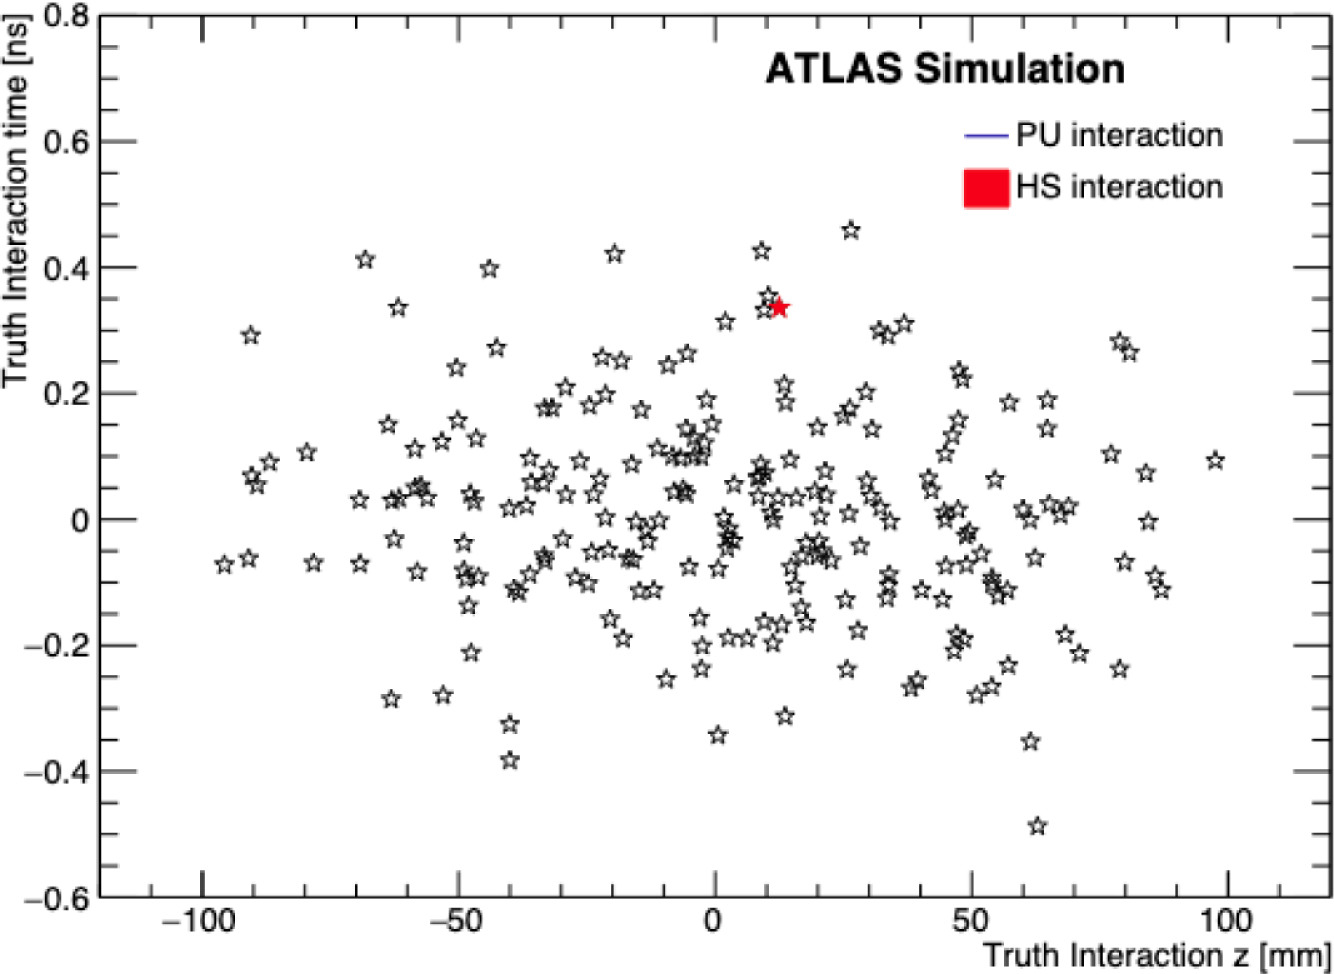
\includegraphics[width=.8\textwidth]{Images/intro/events_pileup_HL_LHC.jpg}
%     \caption{Visualization of the pile-up of events inside ATLAS, using simulation data (PUT SOURCE AND MORE EXPLANATIONS (what is HS?))}
%     \label{fig:events_pileup}
% \end{figure}


\section{Low Gain Avalanche Detectors}

\marginpar{\flushleft Add other image/photo of LGAD}

To provide accurate timing information, silicon detectors were chosen as the active element for the HGTD.

\subsection{Working principles of silicon sensors}

The core of a silicon sensor consists of a junction between two differently doped layers (Figure \ref{fig:p-n_junction_reverse_bias_voltage}), which means that small concentrations of impurities with either higher atomic number ($n$-type) or lower ($p$-type) are introduced inside the crystals.
This forms a $pn$-junction and when a voltage is applied with positive potential on the $n$-side and negative on the $p$-side (reverse bias) the volume between the two layers is depleted of mobile charges and becomes an insulator with an internal electric field.

%%% FIGURE WITH MINIPAGE (for side caption)
\begin{figure}[!h]
    \begin{minipage}[c]{.25\linewidth}
        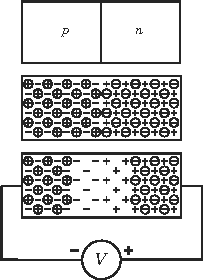
\includegraphics[width=1\linewidth]{Images/LGADs/p-n junction with voltage.png}
    \end{minipage}
    \hfill
    \begin{minipage}[c]{.6\linewidth}
        \caption{\\Top: adjacent regions of $p$-doping (left) and $n$-doping (right) forming a $pn$-junction.\\
        Middle: the circled mobile charges (holes for $p$-type and electrons for $n$-type) balanced by the charge of atomic cores.\\
        Bottom: When an external (reverse) voltage is applied to the junction an electric field builds up in the central region \cite{10.1093/acprof:oso/9780198527848.003.0001}.}
        \label{fig:p-n_junction_reverse_bias_voltage}
    \end{minipage}
\end{figure} 

When a charged particle traverses this depletion layer it frees up electron-hole pairs, which move to the electrodes and can be measured as a pulse in the electric potential.

Generally, silicon detectors provide some advantages over other type of detectors. Due to the lower energy required to produce electron-hope pairs the energy resolution improves. Compared to gas detectors, for example, silicon has a much higher density, allowing detectors to take measurements in considerably thin layers.

On the other hand, this type of device has typically higher manufacturing costs and suffers more considerably from radiation damage.


\subsection{Signal generation by charged particles}

some explanation of the charge distribution that is expected: Landau distribution (appendix)

\subsection{LGADs}

\begin{figure}[!ht]
    \begin{minipage}[c]{.45\linewidth}
        \includegraphics[width=1\linewidth]{Images/LGADs/LGADs_schema_of_work.png}
    \end{minipage}
    \hfill
    \begin{minipage}[c]{.4\linewidth}
        \caption{Cutaway view of an LGAD, not to scale. The depletion region makes the majority of the volume of the sensor, and above it, lies the avalanche region. On the left of the picture there is a qualitative plot of the electric field along the vertical axis of the sensor. From \cite{cernTechnicalDesign}.}
        \label{fig:LGADs_schema}
    \end{minipage}
\end{figure} 

A particular type of silicon sensors are Low Gain Avalanche Detectors (LGAD), an example is shown in Figure \ref{fig:LGADs_schema}. The major innovation over "standard" silicon sensors is an additional $p$-type layer below the $n+$ electrode. This creates a high electric field region which leads to an avalanche effect\footnote[2]{When electrons acquire enough energy they can create new electron-hole pairs ('impact ionization'), which can themselves create new pairs and initialize a multiplication chain that leads to an enhanced signal} of the electrons. This effect produces a gain of around $~10$. \marginpar{\flushleft source} 

The intrinsic multiplication inside LGADs can mitigate the signal degradation caused by radiation damage, however, 

\subsubsection{Time Resolution}

Major factors determining the time resolution of the sensors.

\begin{equation}
    \sigma^2 = \sigma_{TimeWalk}^2 + \sigma_{Jitter}^2 + \sigma_{Landau}^2
\end{equation}





%%% NOT UPDATED ANYMORE, LOOK AT THE EXCEL FILE, I MIGHT DELETE THIS LATER
%%% I have to reorganize these and associate them with the more accurate descriptions
% device name:        vendor:        sensor ID:            fluence:    irradiation type:    type:        board name:    channels:
% CNM-W4              CNM          CNM-R15973-W4-D168      unirradiated      -             single pad     JSI-B12      1
% CNM-W5              CNM          CNM-R15973-W5-D138      unirradiated      -             single pad     JSI-B14      1
% CNM-W3-2.5E15       CNM          CNM-R15973-W3-D29       $\num{2.5e15}     neutron       single pad     JSI B5       1
% CNM-W5-1.5E15       CNM          CNM-R15973-W5-D29       $\num{1.5e15}     neutron       single pad     JSI PP1      1
% USTC2.1             USTC         USTC2.1-W17-P6-A          0                -             2x2           CERN-3       1,2
% USTC2.1 IRRADIATED (MISSING)
% IMEv3-W12-C2         IHEP        IMEv3-W12-C2-2-2          0               -              2x2          CERN-1       channels 1,2
% IMEv3-W12-C3         IHEP        IMEv3-W12-C3-1-4 (and 5)  0               -              1x3          CERN-1       channles 3,4  (small GR), bonded
% CERN2-CH0-IMEv3-W12  IHEP        IMEv3-W12-B2-2-9-1       1.5e15           neutron        2x2 sensor    CERN-2       channels 1,2,3
% CERN2-CH1-IMEv3-W12  IHEP 
% CERN2-CH2-IMEv3-W12  IHEP 
% CERN2-CH4-IMEv3-W16  IHEP        IMEv3-W16-Q4-D4-1-4      1.5e15           neutron        1x3          CERN-2       channel:  2(?)
% JSI-B6-IMEv2-W7-1E14    IHEP       W7-II-C2-1-7 IMEv2-W7Q2    1e14          proton        single       JSI-B6
% JSI-PP4-IMEv2-W7-6.5E14 IHEP       W7-II-C2-1-7 IMEv2-W7Q2    6.5e14        proton        single       JSI-PP4
% JSI-B7-IMEv3-W16-8E14   IHEP       IHEP-IMEv3-W16_Q4_D3_1-4   8e14          (unsure)        single       JSI-B7
% JSI-B13-IMEv3-W16-2.5E15 IHEP      IHEP-IMEv3-W16_Q4_E3_1-4   2.5e15       (unsure)      single        JSI-B13
                 